
Também conhecido como abaixador de tensão, a principal característica dos conversores buck é o controle da corrente na saída, conforme ilustra a figura \ref{cb}.

\begin{figure}[h]
\center
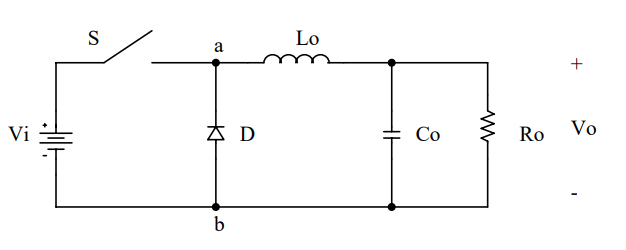
\includegraphics[scale=0.55]{imagens/circuito_buck.png}
\caption{Estrutura do conversor Buck.}\label{cb} 
\caption*{Fonte: Introdução aos conversores CC-CC (2001)}
\end{figure}
 
O seu funcionamento pode ser  descrito em duas etapas. Primeiro, com a chave $S$ em condução, i.e., no período $D \cdot T_s$, a fonte $V_i$ energiza o circuito RLC. No momento em que a chave $S$ abre, no período $\left( 1-D \right) T_s$, o circuito garante inércia da corrente sobre a saída.

Sabendo que a tensão média sobre o atuador, idealmente, é nula, podemos determinar 
\begin{align*}
    V_{o} &= V_{ab,med} =  \frac{1}{T_{s}}\int_{o}^{DT_{s}}V_{i}dt\\
	  &\implies \frac{V_{o}}{V_{i}} = D
.\end{align*} Ou seja, novamente temos uma relação linear entre a razão cíclica e o ganho estático.

A figura \ref{g3b} ilustra o comportamento da tensão e da corrente nos diversos componentes da carga do conversor buck.

\begin{figure}[h]
\center
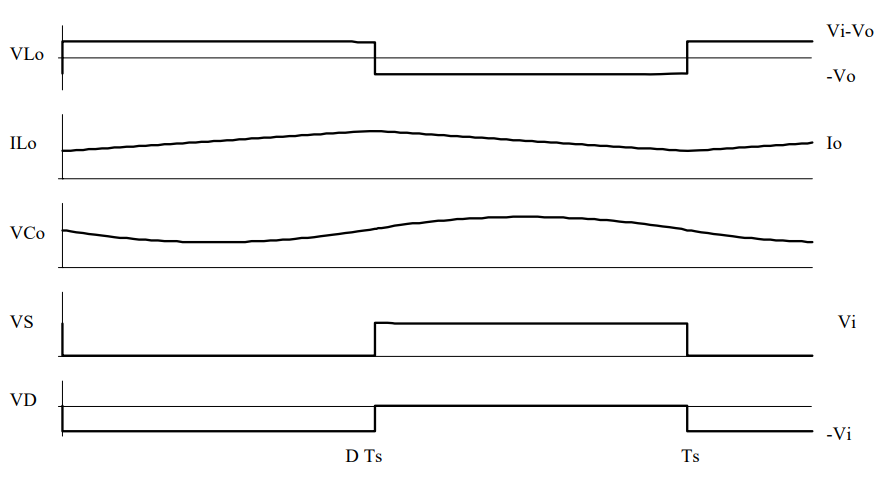
\includegraphics[scale=0.55]{imagens/grafico3_buck.png}
\caption{Formas de onda do conversor Buck.}\label{g3b} 
\caption*{Fonte: Introdução aos conversores CC-CC (2001)}
\end{figure}

De forma similar ao que foi visto nos retificadores, o conversor buck também pode operar em condução contínua, descontínua ou crítica, quando encontra-se na iminência de trocar seu modo de operação.

De modo geral, o conversor Buck está limitado à magnitude da tensão da entrada, mas não tem grande impacto sobre a corrente da saída, i.e., não a distorce muito, ainda que chaveie sempre a corrente fornecida pela alimentação.

